\documentclass[a4paper]{article}

\usepackage{amsmath}
\usepackage{enumitem}

\usepackage{caption}
\usepackage{subcaption}

\usepackage{graphicx}
\author{Kennard Ng and Luo Wen Han}
\title{Project 3: Seam Carving}

\begin{document}
	\maketitle
	
	We use seam carving for image resizing. Ideally, we want to preserve important information in the image. We do this by carving out parts of the image that are redundant i.e. carry the least information. 
	
	More specifically, we carve out seams of pixels from the image. A seam is defined as a path of pixels from one side of an image to its opposing side. In our task, we perform a horizontally resizing of the image where we remove vertical seams i.e. a path of pixels from the top to the bottom of the image, that carry the least amount of important information about the image. 
	
	\section{Background}
	
	Formally, we represent the image as a Hidden Markov Model(HMM). Suppose the image has $r$ rows and $c$ columns, where each pixel is the parent of every other pixel in the next row. Let the each pixel be indexed by $i,j$, and have a hidden random variable $Z_{i,j}$ that denotes the importance of the pixel and  an observed variable $X_{i,j}$ that is conditioned on the $Z_{i,j}$. More specifically, the relationship between variables $Z_{0,1}, Z_{1,1}, Z_{2,1}$ and $X_{1,1}$ is as follows: 
	\begin{figure}[ht]
		\centering
		\includegraphics[width=0.5\linewidth]{images/relationship}
		\caption{Hidden Markov Model Example}
		\label{fig:relationship}
	\end{figure}
	
	From Figure \ref{fig:relationship}, we see that every variable in the HMM is conditionally independent of other nodes in the graph given its parent. In our setting, $Z_{i,j}$ is the parent of every other random variable in the next row i.e. $Z_{i+1,k}$ for $k \in \left\{1, \cdots, m\right\}$. The edges of the HMM are defined by the transition probabilities between hidden states $p(Z_{i,j}|Z_{i+1,k})$ and the emission probability $p(Z_{i,j}|Z_{i,j})$.
	
	We can parameterize a seam as an extended version of the HMM given in Figure \ref{fig:relationship}. The joint probability of a single seam can be expressed as a HMM in a factorized form based on the conditional independence: 
	
	\begin{equation}
		\Pr(X, Z)=\prod_{i=0}^{r-1} \prod_{j=0}^{c-1} \prod_{k=0}^{c-1} \Pr\left(z_{i,j} | z_{i,k}\right) \Pr\left(x_{i,j} | z_{i,j}\right).
		\label{eqn:joint}
	\end{equation}
	
	In our task, we want to find the minimum a posterior of hidden states $\mathbf{Z}$ given the observations $\mathbf{O}$ where $\mathbf{O}$ is the gradients of the pixel. Given that the gradients can be zero for a single pixel, which collapses the values of joint probability of the seam to zero if we were to naively use Equation \ref{eqn:joint}, we parameterize the problem in terms of its log linear form:
	
	\begin{equation}
	\log\Pr(X, Z)=\sum_{i=0}^{r-1} \sum_{j=0}^{c-1} \log\Pr\left(x_{i,j} | z_{i,j}\right) + \sum_{k=0}^{c-1} \log\Pr\left(z_{i,j} | z_{i,k}\right),
	\end{equation}
	
	The log transition probability is given by: 
	\begin{equation}
		\log\Pr\left(Z_{i,j} | Z_{i,k}\right)=\left\{\begin{array}{ll}{1} & {\text { if }\left|j - k\right| \leq 1} \\ {\infty} & {\text { else }}\end{array}\right. , 
	\end{equation}
	which implies that we the minimum configuration would only involve the three nearest pixels on the lower row i.e. $k \in \left\{j-1, j, j+1\right\}$, and we represent the log emission probability as:
	\begin{equation}
		\log\Pr\left(X_{i,j} | Z_{i,j}=z'\right)=E_{i,j}(z') = \eta X_{i,j},
	\end{equation}
	
	where $E$ is the energy map of the image, which we set to be the gradients $X$ multiplied by a normalizing constant $\eta$. Given that we are finding the minimum configuration, we can simply drop $\eta$ and use the gradient values. 
	
	\section{Vertibi Algorithm}
	
	We use the Vertibi Algorithm in our formulation. The Vertibi algorithm is based on dynamic programming and at each vertibi $v_i$, it computes the vertibi which is the minimum configuration given the previous $i-1$ hidden states and the $i$ observations. It uses the following recursive formulation:
	
	\begin{equation}
		v_i = \min_{0\cdots c-1} v_{i-1}\text{Pr}_{em}\text{Pr}_{tr},
		\label{eqn:vertibi}
	\end{equation}
	where $\text{Pr}_{em}$ and $\text{Pr}_{tr}$ represents the emission probability of a pixel in the current row and the transition probability from the pixel in the higher row (in the previous iteration) that gives the minimum configuration for $v_{i-1}$ into the pixel in the present row, respectively. We formulate \ref{eqn:vertibi} in a log-linear form as well:
	\begin{equation}
		v_i = \min_{0\cdots c-1} v_{i-1} + \log\text{Pr}_{em} + \log\text{Pr}_{tr},
	\end{equation}	
	and each seam has a final vertibi $v_{r-1}$, where a seam begins from a pixel along the top row of the image. At each iteration, we have $c_t$ seams, where $c_t$ is the number of columns of the image at iteration $t$. We select the seam with the minimum vertibi $v_{r_{t-1}}$  at each iteration and remove it, by shifting the pixels on the right of the seam to the left by one pixel. 
	
	The pseudo code of our implementation of the Seam Carving algorithm is given below: \\
	
	\textbf{Seam Carving Algorithm}
	\begin{enumerate}[noitemsep]
		\item Repeat for $T$ iterations until desired image size:
		\begin{enumerate}[noitemsep]
			\item Let the iteration be $t$, number of rows of the image be $r$, and the number of columns be $c_t$.
			\item Run Vertibi algorithm and backtrack from the algorithm to get the location of the pixels that form the seam with the minimum vertibi.
			\item Remove the seam pixels by shifting the pixels on the right of the seam to the left.
		\end{enumerate}
	\end{enumerate} 
	
	\textbf{Vertibi Algorithm}
	\begin{enumerate}[noitemsep]
		\item Let the $v_\text{min} = \infty$
		\item For $j = 0, \cdots, c_t-1$, 
		\begin{enumerate}[noitemsep]
			\item Let the starting pixel be the pixel indexed by $0,k$, where $k=j$ initially.
			\item Let $v_0 = x_{0,j}$.
			\item For $i=1, \cdots, r-1$, compute $v_i = v_{i-1}\min_k x_{i,k}$ for $k \in \left\{j-1, 0, j+1\right\}$. 
			\item Update $v_\text{min} = \min(v_{r-1}, v_\text{min})$ 
		\end{enumerate}
		\item Backtrack $v_\text{min}$ and return the pixel locations of the seam with the minimum configuration.
	\end{enumerate}
	
	\section{Qualitative Results}
	
	These are our qualitative results:
	\begin{figure}[ht]
		\centering
		\begin{subfigure}{0.45\linewidth}
			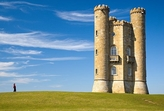
\includegraphics[height=1.5in]{images/image_input}
			\caption{Original Image}
			\label{fig:imageinput}
		\end{subfigure}
		\begin{subfigure}{0.45\linewidth}
			\centering
			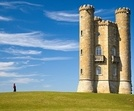
\includegraphics[height=1.5in]{images/image_output}
			\caption{Resized Image}
			\label{fig:imageoutput}
		\end{subfigure}
	\end{figure}
	
	From our results, we see that important parts of the image i.e. the person and the castle have been preserved during the resize operation, where their scale have been preserved. On the other hand, unimportant parts of the iamge i.e. background has been carved away during the resize operation.
	

	
	
\end{document}